\documentclass{article}
\usepackage[UTF8]{ctex}
% Replace `letterpaper' with`a4paper' for UK/EU standard size
\usepackage[a4paper,top=2cm,bottom=2cm,left=3cm,right=3cm,marginparwidth=1.75cm]{geometry}

% Useful packages
\usepackage{amsmath}
\usepackage{mathrsfs,amsmath}
\usepackage{graphicx}
\usepackage[colorlinks=true, allcolors=blue]{hyperref}
\usepackage{graphicx} %插入图片的宏包
\usepackage{float} %设置图片浮动位置的宏包
\usepackage{subfigure} %插入多图时用子图显示的宏包
\usepackage{parskip}
\usepackage{indentfirst} 
\setlength{\parindent}{2em}
\usepackage{hyperref}  
\usepackage{tikz}
\allowdisplaybreaks
\usepackage{multirow}
\usepackage{amsmath}
\usepackage{amsfonts,amssymb} 
\usepackage{xcolor} % 用于显示颜色
\usepackage{listings} % 用于插入代码
\lstset{
	basicstyle          =   \sffamily,          % 基本代码风格
	keywordstyle        =   \bfseries,          % 关键字风格
	commentstyle        =   \rmfamily\itshape,  % 注释的风格,斜体
	stringstyle         =   \ttfamily,  % 字符串风格
	flexiblecolumns,                % 别问为什么,加上这个
	numbers             =   left,   % 行号的位置在左边
	showspaces          =   false,  % 是否显示空格,显示了有点乱,所以不现实了
	numberstyle         =   \zihao{-5}\ttfamily,    % 行号的样式,小五号,tt等宽字体
	showstringspaces    =   false,
	captionpos          =   t,      % 这段代码的名字所呈现的位置,t指的是top上面
	frame               =   lrtb,   % 显示边框
}

\lstdefinestyle{Python}{
	language        =   Python, % 语言选Python
	basicstyle      =   \zihao{-5}\ttfamily,
	numberstyle     =   \zihao{-5}\ttfamily,
	keywordstyle    =   \color{blue},
	keywordstyle    =   [2] \color{teal},
	stringstyle     =   \color{magenta},
	commentstyle    =   \color{red}\ttfamily,
	breaklines      =   true,   % 自动换行,建议不要写太长的行
	columns         =   fixed,  % 如果不加这一句,字间距就不固定,很丑,必须加
	basewidth       =   0.5em,
}

\title{图像处理与可视化 Homework-7 报告}
\author{林子开 21307110161}
\begin{document}
	\maketitle
	\tableofcontents

\section{FFD形变算法}
\subsection{FFD原理简介}
FFD算法的核心想法是:将控制点规则化,并且把控制点的位移产生的影响控制在局部。

FFD的变换公式为:$Y=T(X) = X + Q_{local}(X)$,其中$Q_{local}(X)$表示$X$发生的位移:
\begin{align*}
&Q_{local}(X) = \sum_{i=-1}^{2} \sum_{j=-1}^{2} \varPhi_{i+i_x,j+j_x} \beta_i(u)\beta_j(v) \\
&u = \frac{x-P_{00}[0]}{l_x}-i_x, \; v=\frac{y-P_{00}[1]}{l_y}-j_y \\
&i_x = \left\lfloor\frac{x-P_{00}[0]}{l_x}\right\rfloor, \; j_y = \left\lfloor \frac{y-P_{00}[1]}{l_y} \right\rfloor 
\end{align*}
其中$\varPhi_{i+i_x,j+j_x}$表示$(i+i_x,j+j_x)$处的控制点的位移,$\beta_i,\beta_j$
是分段形式的B-样条核函数。

\subsection{FFD的Python实现}
\lstinputlisting[style = Python,
caption={FFD形变算法}]{FFD.py} 

\section{反向图像变换}

\subsection{反向变换原理简介}
设原始图的像素为$X$,目标图的像素为$Y$,满足$Y=T(X)$。
反向变换算法遍历目标图中的每一个像素坐标$Y(i,j)$,并基于\textbf{反变换}求出在原始图对应的
浮点型坐标$X(p,q)=T^{-1}[Y(i,j)]$,再利用插值得到$X(p,q)$处的灰度值$f(p,q)$,
并把$Y(i,j)$处的灰度值设置为$f(p,q)$。

在本次作业中,反变换是基于FFD形变算法实现的。由用户在\textbf{原图}上选取若干个点,
不妨记作$\{X_1,\dots , X_n\}$,然后指定这些点经过变换后在\textbf{目标图}上所在位置,不妨记作$\{Y_1,\dots,Y_n\}$,
也即在原图上的点$X_1$的坐标$X_1(p,q)$,经过变换后,它的坐标将变成$Y_1$点的坐标$Y_1(i,j)$。

将$\{Y_1,\dots,Y_n\}$映射到最近的规则化控制点$\{Z_1,\dots,Z_n\}$,并设控制点$Z_i$对应的位移为
$X_i(p,q)-Y_i(i,j)$。然后遍历所有的像素点的坐标$Y(i,j)$,基于FFD,找到在原图上的浮点型坐标$X(p,q)$,
进行插值并回填。这样就实现了基于FFD的反变换。

\subsection{反向变换的Python实现}

\lstinputlisting[style = Python,
caption={FFD形变算法}]{backward_transformation.py} 

\subsection{效果测试}
在原图上选取8个控制点,分别位于正方形的四个顶点,以及四条边的中点,如图\ref{1}所示。
位于顶点的控制点向边缘移动,位于四条边中点的控制点向中心移动,如图\ref{2}所示。

\begin{figure}[H]
    \centering
    \subfigure[原图的控制点所处位置]
    {\label{1} 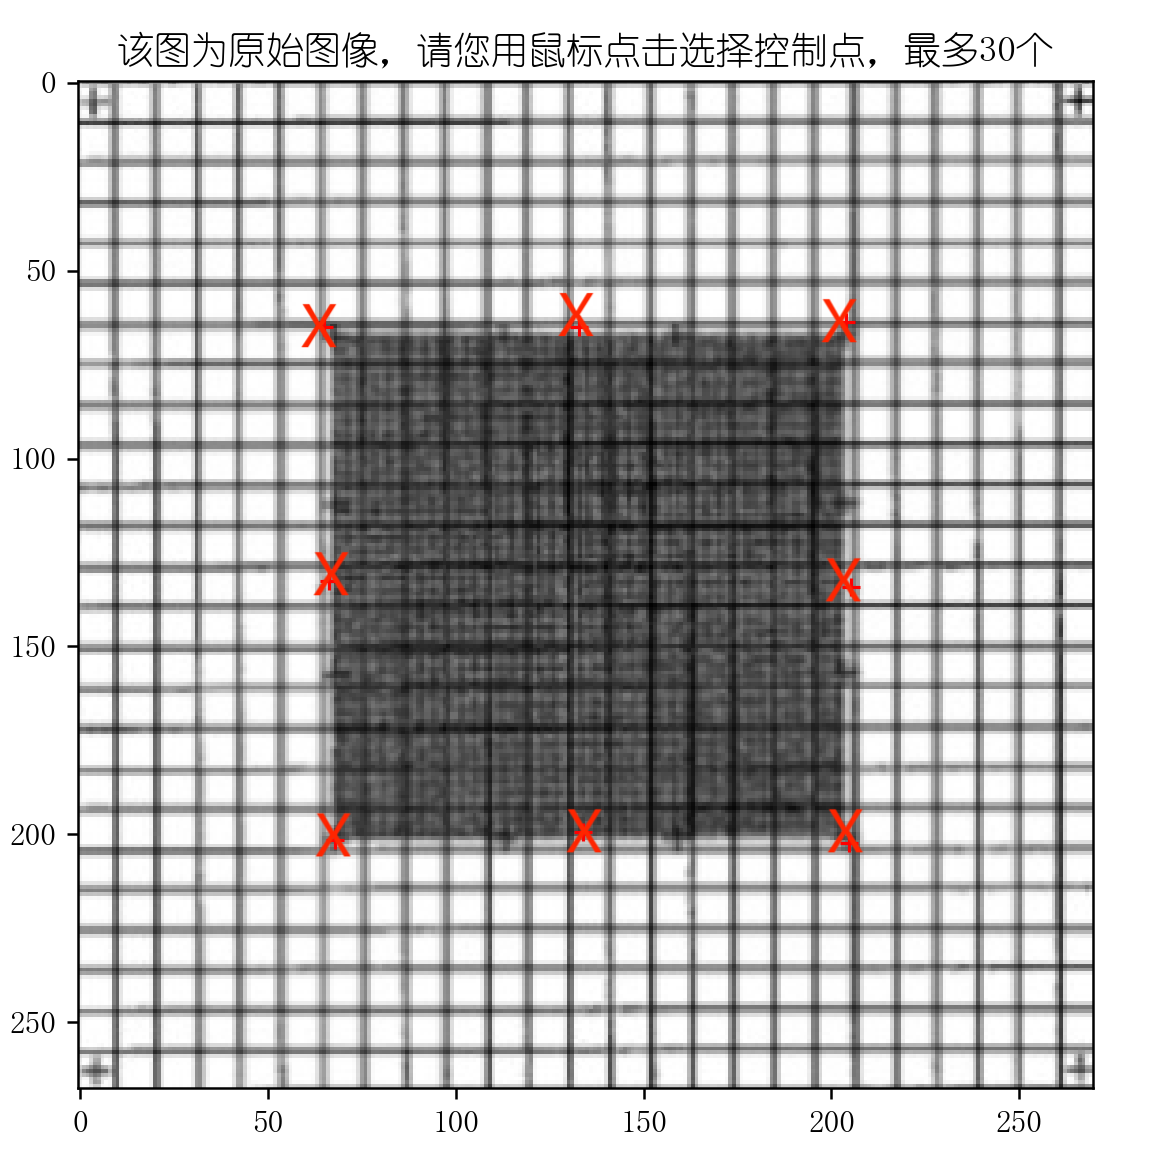
\includegraphics[width=0.45\textwidth]{image//原图选点.png}}
    \,    
    \subfigure[控制点变换后所处位置]
    {\label{2} 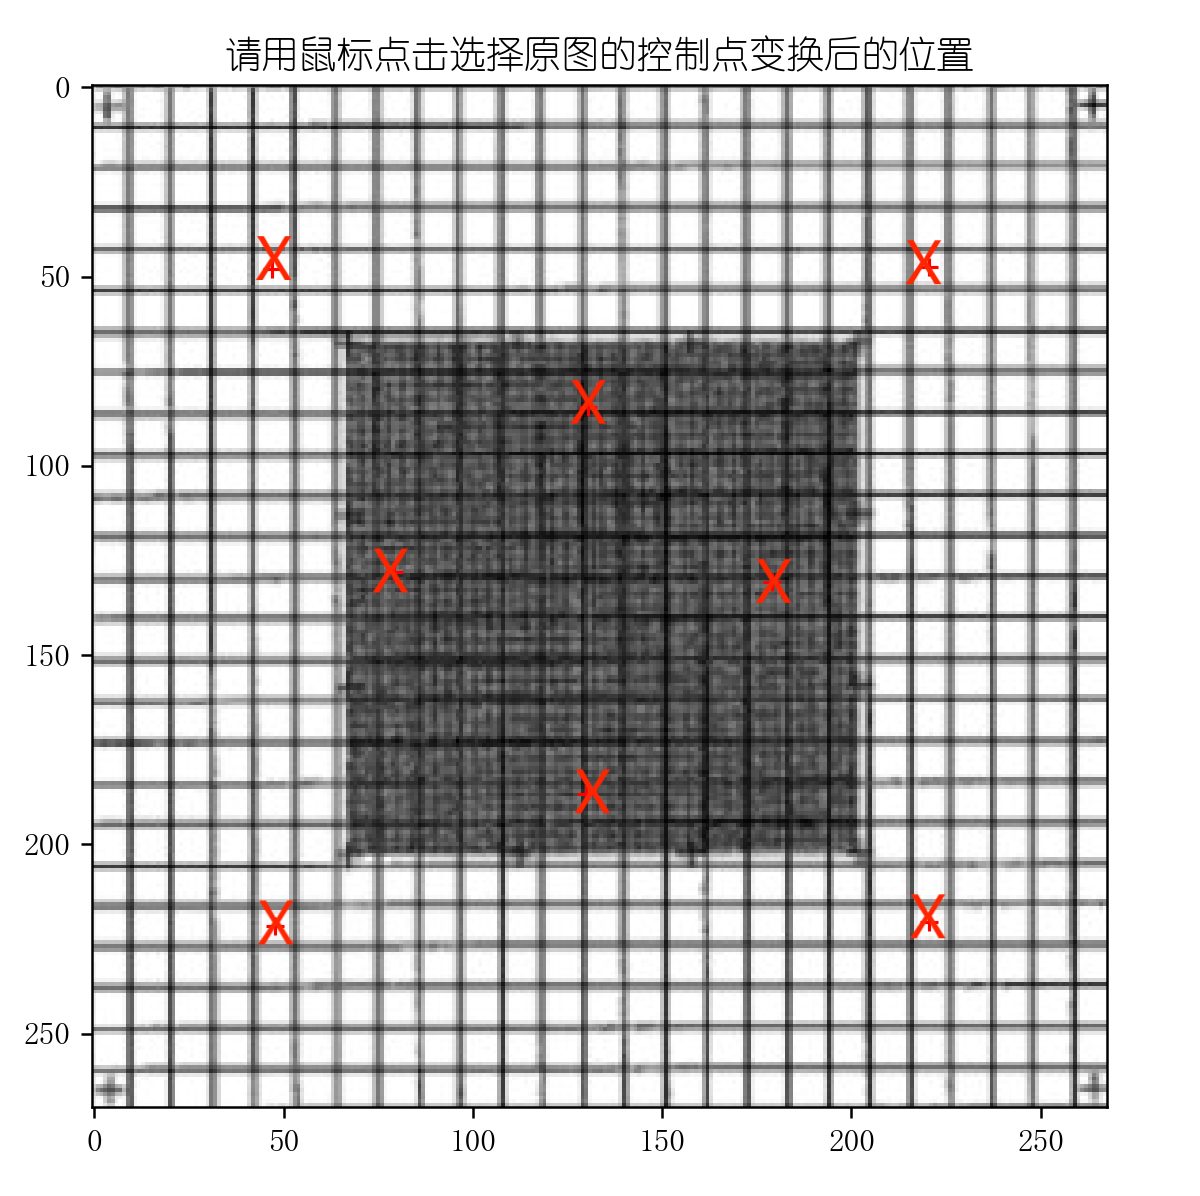
\includegraphics[width=0.45\textwidth]{image//新图选点.png}}
\end{figure}

以下是原图和形变图的对比。可以看出,形变的影响确实被控制在了局部范围内。
\begin{figure}[H]
    \centering
    \subfigure[原图]
    {\label{} 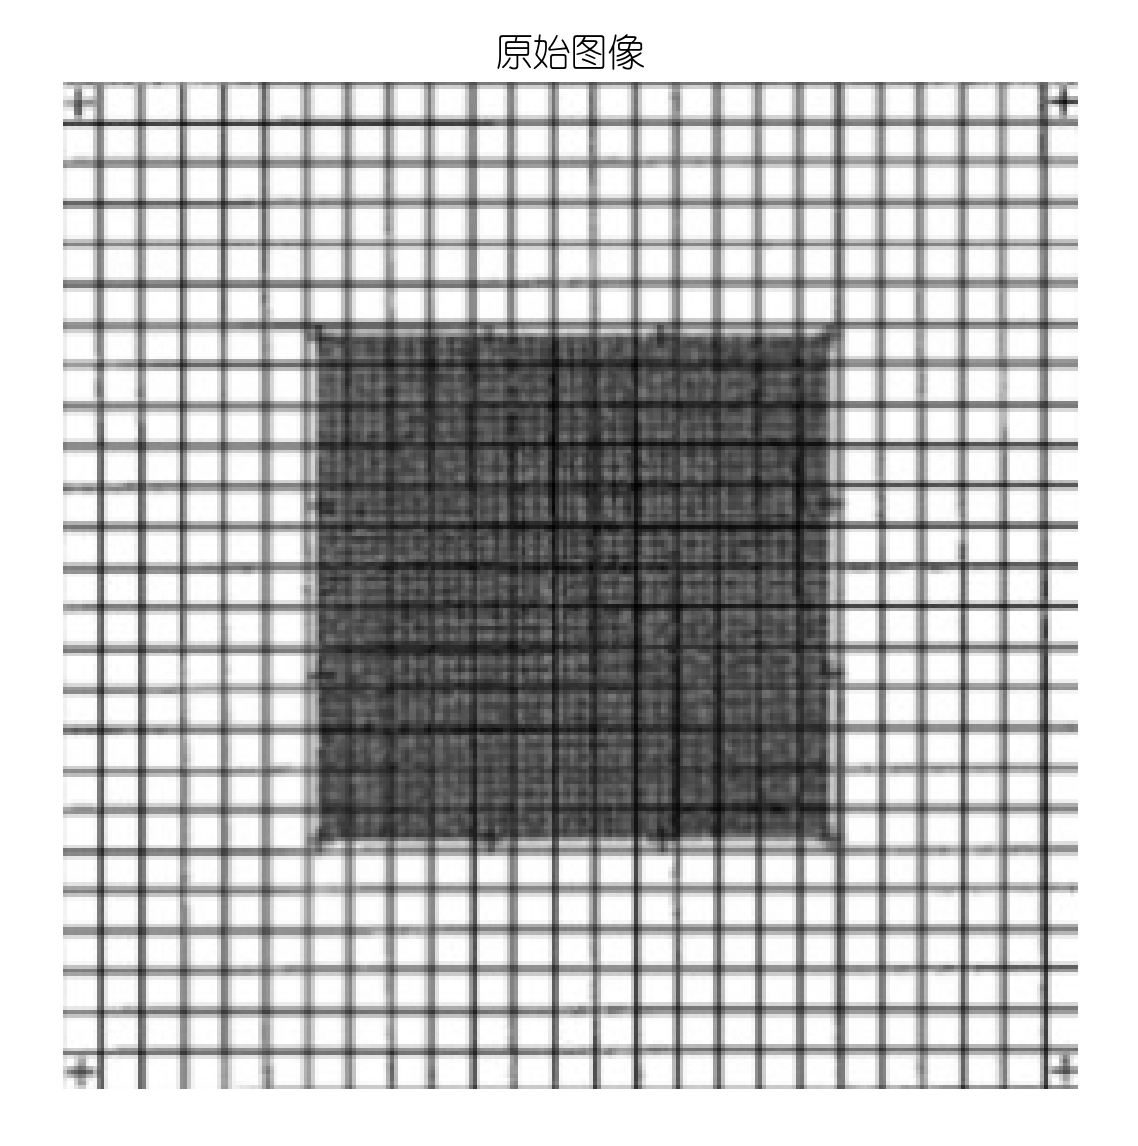
\includegraphics[width=0.45\textwidth]{image//原始图像.png}}
    \,    
    \subfigure[形变图]
    {\label{} 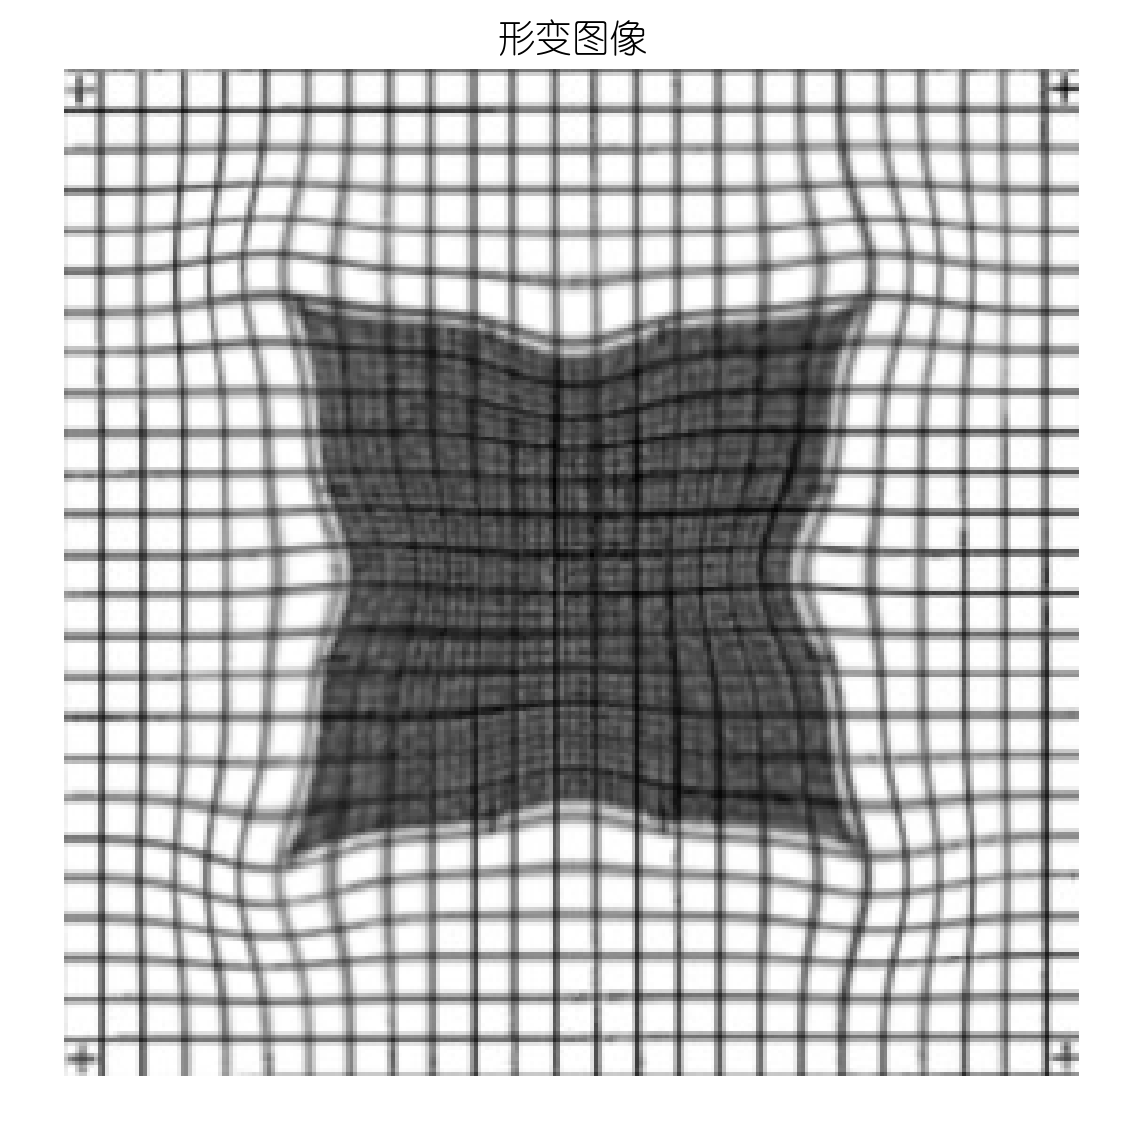
\includegraphics[width=0.45\textwidth]{image//形变图像.png}}
\end{figure}

\end{document}

% \begin{figure}[H]
% 	\centering
% 	{\includegraphics[width=0.35\textwidth]{image//ignorance.png}} 
% 	\caption{} \label{} 
% \end{figure}


% \lstinputlisting[style = Python,
% caption={Python codes},
% label = {efficient},
% linerange={110-125}]{exercise3.py} 


% \begin{figure}[H]
%     \centering
%     \subfigure[patch size = 11]
%     {\label{} 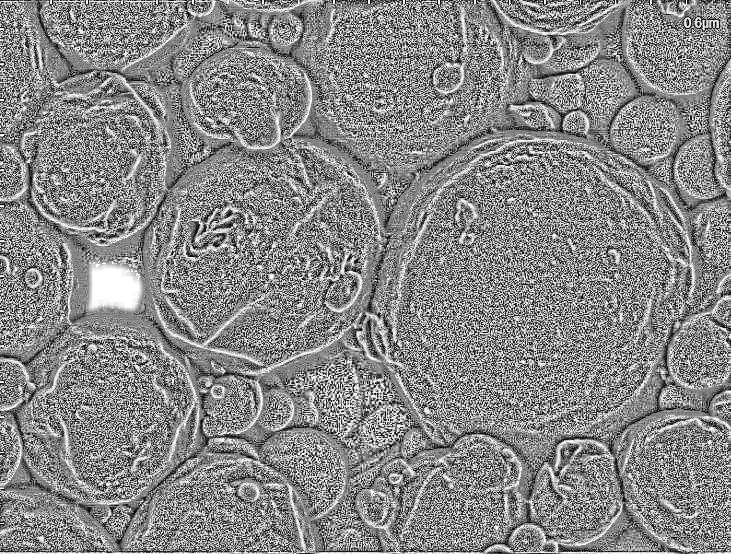
\includegraphics[width=0.49\textwidth]{image//local equalization with patch size = 11.jpg}}
%     \,    
%     \subfigure[patch size = 51]
%     {\label{} 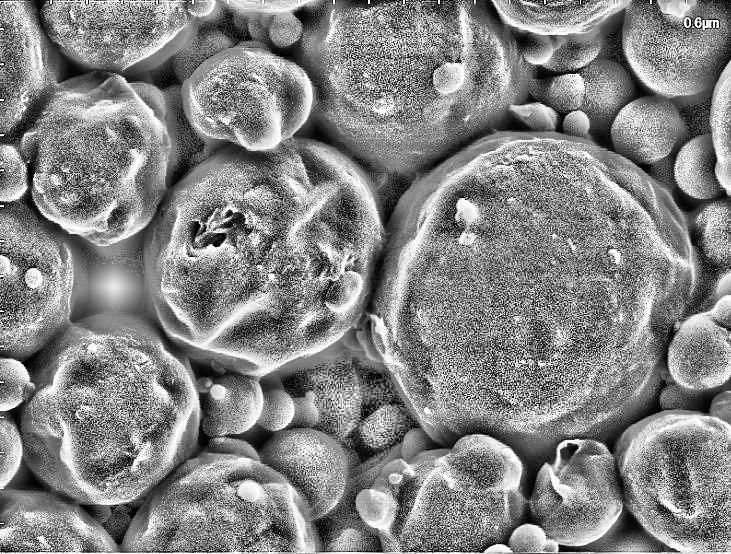
\includegraphics[width=0.49\textwidth]{image//local equalization with patch size = 51.jpg}}
%     \,
%     \subfigure[patch size = 151]
%     {\label{} 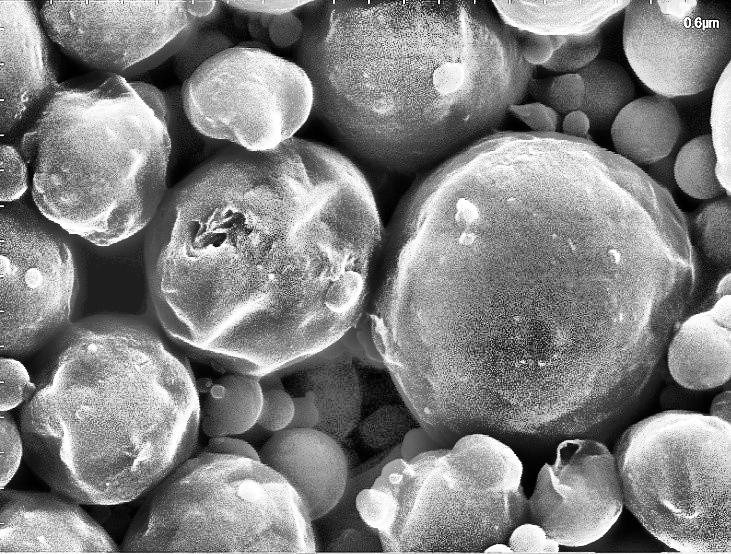
\includegraphics[width=0.49\textwidth]{image//local equalization with patch size = 151.jpg}}
%     \,    
%     \subfigure[patch size = 201]
%     {\label{} 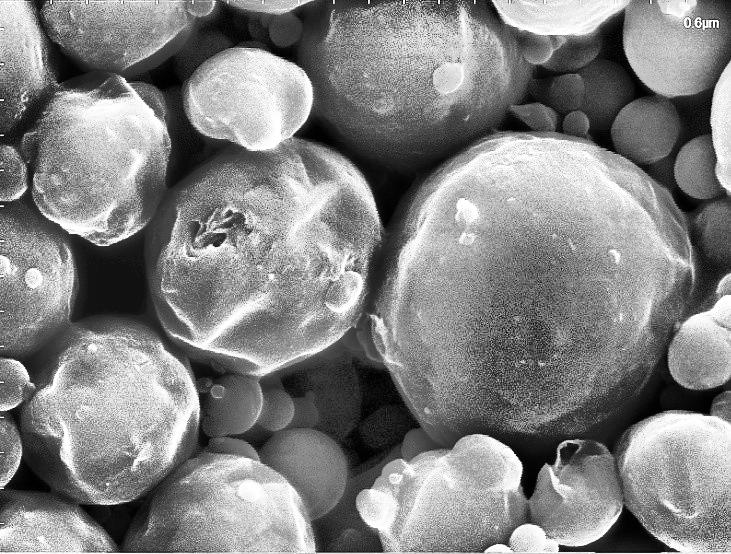
\includegraphics[width=0.49\textwidth]{image//local equalization with patch size = 201.jpg}}
%     \caption{local equalization with different patch sizes}\label{} 
% \end{figure}
